\subsection{Resultados da Rede gerada}

Os dados das Figuras 
\ref{fig:contatos_faixa} e \ref{fig:heat} serão utilizados como \textit{inputs} do Modelo de Configuração Ponderado, onde aquele vai ser usado para construir a distribuição empírica do grau de cada nó de cada faixa etária e este será usado como parâmetros de uma multinomial para estabelecer quantas ligações vão para cada faixa etária. A partir disso e dado um valor de $p$ 
(parâmetro que aumenta o coeficiente de agrupamento)
será construída a rede para acontecer a simulação da epidemia. As características dessa rede são mostradas na Tabela \ref{table:rrede} e na Figura \ref{fig:regressao}
mostra-se como evolui o agrupamento com o incremento de $p$, que cresce com $C \propto p^{\alpha}$, tanto o agrupamento médio quanto o total no qual $\alpha_{medio } = 0.46$ e $\alpha_{medio } = 0.55$. Após a aplicação do algoritmo foi recolhido os dados da rede e observou-se que para qualquer valor de $p$ a distribuição de graus tinha a mesma distribuição que a encontrada pela Figura \ref{fig:contatos_faixa} a partir do teste de Kolmogorov-Smirnov (Figura \ref{fig:comparacao}) \cite{manual} e na Tabela \ref{tab:pvalor} mostra a lista dos P-valores para cada valor de $p$. Na Figura \ref{fig:modelo}
mostra-se a diferença absoluta ao final do algoritmo da proporção de conexões de cada faixa etária em comparação com a Figura \ref{fig:heat}, tendo uma diferença maior entre as conexões com faixa etária 1.


\begin{table}[H]
    \centering
    \captionsetup{font=normalsize,skip=0.8pt,singlelinecheck=on,labelsep=endash}
    \caption{P-valores para diferentes valores de $p$.}
    \begin{tabular}{|c|c|c|c|c|c|}
    
    \hline
    \multirow{2}{*}{$p$} & \multicolumn{5}{c|}{Faixa Etária} \\ \cline{2-6} 
     & 1 & 2 & 3 & 4 & 5 \\ \hline
    0 & 1.0 & 0.992 & 0.975 & 0.851 & 0.434 \\ \hline
    \rowcolor{Gray}
    0.5 & 1.0 & 0.903 & 1.0 & 0.092 & 0.146 \\ \hline
    1.0 & 1.0 & 0.988 & 1.0 & 0.772 & 0.993 \\ \hline
    \end{tabular}
    \label{tab:pvalor}
\end{table}

\begin{figure}[H]
    \centering
    %PIF27092023
    \captionsetup{font=normalsize,skip=0.8pt,singlelinecheck=on,labelsep=endash}
    \caption{Agrupamento da rede em função de $p$}
    %PIF27092023 É possível apagar o enquadramento branco?        
    %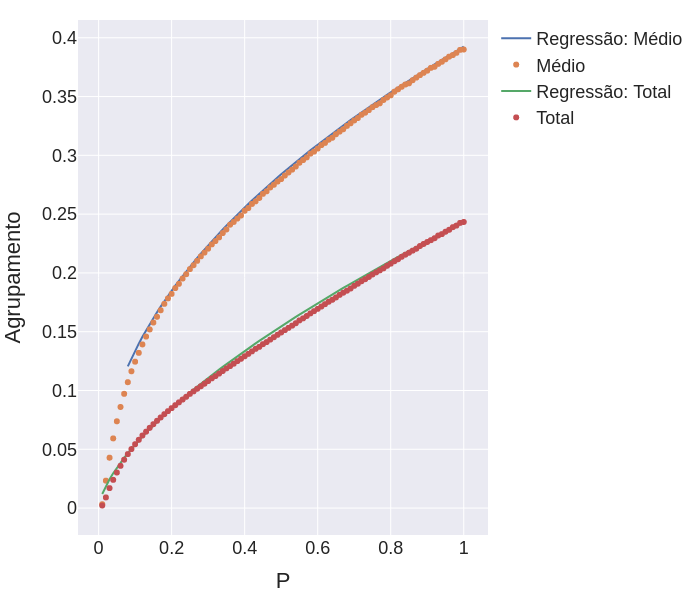
\includegraphics[scale= 0.5]{figuras/clustering_vs_p.png}
    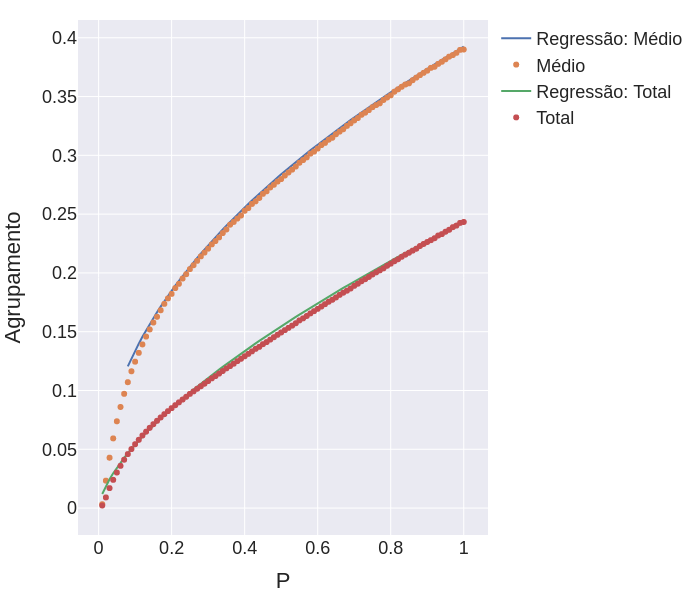
\includegraphics[scale= 0.5]{figuras/clustering_vs_p.png}
    \captionsetup{font=small,justification=justified}    \caption*{Evolução do agrupamento da rede em função 
    do incremento do valor de $p$, foi utilizada uma regressão linear para saber qual a função que rege encontrando $C \propto p^{\alpha}$.\\Fonte: Autor}
    \label{fig:regressao}
\end{figure}


\begin{figure}[H]
    \centering
    
    \captionsetup{font=normalsize,skip=0.8pt,singlelinecheck=on,labelsep=endash}
    \caption{Resultados da proporção de conexões entre faixas}
    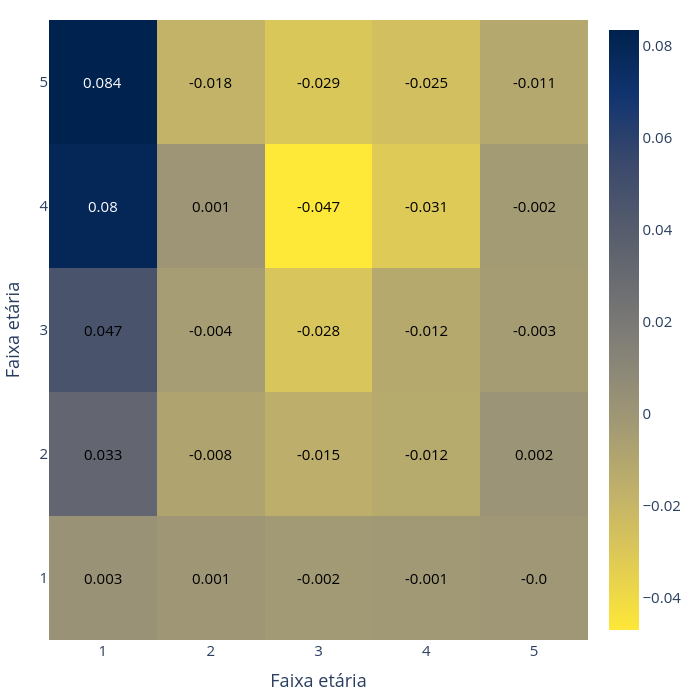
\includegraphics[scale= 0.4]{figuras/modelo.png}
    \captionsetup{font=small,justification=justified}
    \caption*{ A figura mostra a diferença absoluta entre a matriz de proporções de conexões entre as faixas etárias do modelo e do encontrado no POLYMOD essa diferença se mantém constante independe do valor de $p$.}
    \label{fig:modelo}
\end{figure}


\begin{table}[H]

  %PIF15102023
%  \centering
%  \captionsetup{margin={9pt,14pt},font=normalsize,skip=0.5pt,labelsep=endash}
\captionsetup{font=normalsize,skip=0.8pt,singlelinecheck=on,labelsep=endash}
\caption{Métricas das redes geradas.}
  \centering
  \hspace*{-\leftmargin}\begin{tabular}{lcccccc}

    \hline

    \multicolumn{1}{l|}{ \textbf{\shortstack{$p$}}} & 
    \multicolumn{1}{c|}{\textbf{\shortstack{Grau \\ Médio}}}  & 
    \multicolumn{1}{c|}{\textbf{\shortstack{Grau \\ Mediano}}} &
    \multicolumn{1}{c|}{\textbf{\shortstack{Desvio \\ Padrão \\ Grau}}} &
    \multicolumn{1}{c|}{\textbf{\shortstack{Agrupa-\\mento \\ Médio}}} & 
    \multicolumn{1}{c|}{\textbf{\shortstack{Menor \\ Caminho \\ Médio}}} & 
    \multicolumn{1}{c}{{\shortstack{\textbf{Diâmetro}}}}     \\

    \hline
    
    0 & 13.24(0.23) & 10.024(0.19) & 10.38(0.22) & 0.01(0.00) & 3.26(0.02) & 6.778(0.48) \\
    \rowcolor{Gray}
    0.5 & 13.27(0.22) & 10.037(0.21) & 10.39(0.22) & 0.21(0.01) & 3.39(0.02) & 7.123(0.41) \\
    
    1.0 & 13.27(0.22) & 10.034(0.22) & 10.40(0.22) & 0.31(0.01) & 3.51(0.03) & 7.333(0.54) \\
    \hline

    
\end{tabular}

\caption*{Com o incremento de $p$ houve um aumento significativo no agrupamento, como esperado, o que acarretou em um aumento do menor caminho médio e do diâmetro da rede.}
\label{table:rrede}
\end{table}

\begin{figure}[H]
    \centering
    \captionsetup{font=normalsize,skip=0.8pt,singlelinecheck=on,labelsep=endash}
    \caption{Distribuição de Graus $p = 1.0$}
    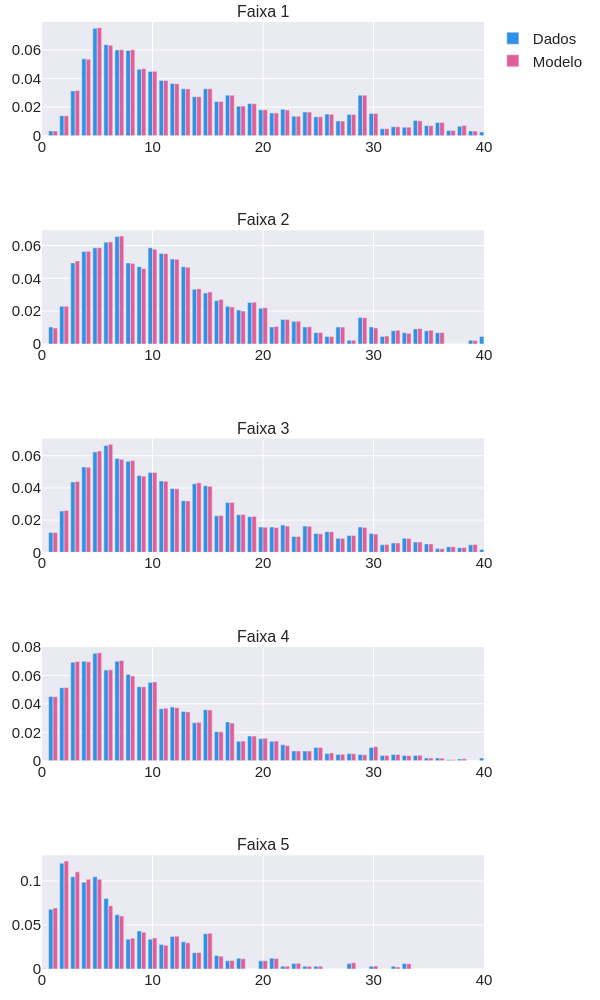
\includegraphics[scale= 0.4]{figuras/comparacao.png}
    \captionsetup{font=small,justification=justified}
    \caption*{Comparação de como fica a distribuição de graus comparando modelo com $p = 1.0$ com dados do POLYMOD, é possível ver que a Faixa etária 4 e 5 são as mais afetadas mas apresentam a mesma distribuição de acordo com o Teste.\\Fonte: Autor}
    \label{fig:comparacao}
\end{figure}
